\documentclass[10pt]{article}
\usepackage{calc}
\usepackage{subfiles}
\usepackage{hyperref}
\usepackage[utf8]{inputenc}
\usepackage[swedish]{babel}
\usepackage[margin=2cm]{geometry}
\usepackage{scrextend}
\usepackage[backend=bibtex,sorting=none,style=numeric,natbib=true]{biblatex}
\usepackage{graphicx}
\graphicspath{ {images/} }
\usepackage{filecontents}
\selectlanguage{swedish}


\addbibresource{../references.bib}

\usepackage{xifthen}
\usepackage{enumitem}
\usepackage{scrextend}
\newcounter{switchcase}

\newcommand{\ifequals}[3]{\ifthenelse{\equal{#1}{#2}}{\stepcounter{switchcase} #3}{}}
\newcommand{\case}[2]{#1 #2} % Dummy, so \renewcommand has something to overwrite...
\newenvironment{switch}[1]{
  %Executed at \begin{switch}
  \setcounter{switchcase}{0}
  \renewcommand{\case}{\ifequals{#1}}
}{
 % Executed at \end{switch}
\ifthenelse{\equal{\value{switchcase}}{0}}{
  \PackageError{ProjectDefinitions}{Could not find given definition}{}}{}
}

\newcommand{\definition}[1]
{
  \begin{switch}{#1}
    \case{Cachning}{\item [\textbf{#1}]
      Temporär lagning av data för snabb åtkomst.}
    \case{Instans}{\item [\textbf{#1}]
      En spelsession som startas från UI-applikationen och spelare kan gå med i för att spela spelet tillsammans.}
    \case{IoT-backend}{\item [\textbf{#1}]
      Existerande system som kan dirigera data mellan många uppkopplade enheter.}
    \case{Kontroll-applikation}{\item [\textbf{#1}]
      Applikation som körs på en mobil eller surfplatta och tar input från användare.}
    \case{Progressive Web Apps}{\item [\textbf{#1}]
      Förkortat PWA, är ett mellanting mellan en hemsida och en applikation.
      Med en PWA behöver man inte ladda ner en app, men den ger viss funktionalitet som appar har. \cite{bib-pwa}}
    \case{Resurs}{\item [\textbf{#1}]
      Media som används i spelet, t.ex. bilder och ljud.}
    \case{Sensor}{\item [\textbf{#1}]
      En sensor som sitter på kontroll-applikationen och inte är en pekskärm, t.ex. en accelerometer.}
    \case{Server-klient-modell}{\item [\textbf{#1}]
      Struktur på ett system där någon enhet tillhandahåller resurser, information eller tjänster och flera andra enheter interagerar med denna.}
    \case{Spelläge}{\item [\textbf{#1}]
      En utökning av grundspelet som definierar speciella regler och spelmekanik.}
    \case{Spelmekanik}{\item [\textbf{#1}]
      Regler och möjligheter som definierar ett spel.}
    \case{Tunn klient}{\item [\textbf{#1}]
      Specialfall av server-klient-modell där mycket få beräkningar sker på klienten.}
    \case{UI-applikation}{\item [\textbf{#1}]
      Applikationen som kör spelet och visar spelplanen.}
    \case{Use Case Map}{\item [\textbf{#1}]
      Diagram som illustrerar hur olika händelser interagerar med arkitekturen. \cite[p.~30--33]{bib-architecture-primer}}
    \case{Scrum-board}{\item [\textbf{#1}]
      En tavla med post-it lappar som innehåller aktiviteter som ska göras under
      projektet. Detta komplementeras med olika kolumner i tavlan såsom planerad, pågående,
      testning och utgåva. Dessa bestämmer i vilket stadie lapparna befinner sig i.}
    \case{Burndown-chart}{\item [\textbf{#1}]
      En graf som visar hur många timmar medlemmarna har lagt ner i förhållande till vad som krävs för att hinna med projektet.}
    \case{Acceptanstest}{\item [\textbf{#1}]
      Slutgiltiga testet som kund utför för att se att produkten lever upp till förväntningarna.}
    \case{Enhetstest}{\item [\textbf{#1}]
      Testa varje enhet så den fungerar när den är färdig.}
    \case{Integrationstest}{\item [\textbf{#1}]
      Testa att en ny enhet som läggs till i projektet fungerar som den ska tillsammans med de andra enheterna.}
    \case{Kund}{\item [\textbf{#1}]
      Cybercom Sweden.}
    \case{Regressionstest}{\item [\textbf{#1}]
      Testa ny kod enligt gamla parametrar för att säkerställa att ingen funktionalitet försvunnit.}
    \case{Systemtest}{\item [\textbf{#1}]
      Test för att säkerställa att enheten uppfyller kraven för projektet.}
    \case{Cybercom}{\item [\textbf{#1}]
      Kortare variant av Cybercom Sweden, företaget produkten utvecklas åt.}
    \case{Enkäten}{\item [\textbf{#1}]
      Den enkät som ska användas för att utvärdera användarupplevelsen, se avsnitt  3.3 Demo och enkät.}
    \case{Kvalitet}{\item [\textbf{#1}]
        I likhet med IEEE 730 definierar denna rapport kvalitet som konformitet till projektets krav. \cite{ieee730}}
    \case{Projektet}{\item [\textbf{#1}]
        Processen att framställa en produkt åt Cybercom Sweden.}
    \case{Software Quality Asssurance}{\item [\textbf{#1}]
    	Förkortat SQA, är en samling aktiviteter som bedömmer lämpligheten och inger förtroende
    	för utvecklingsmetodiken som används.}
    \case{SQA-process}{\item [\textbf{#1}]
      I likhet med IEEE 730 definieras en SQA-process som aktiviteten att samla underlag för att med säkerhet ta
      beslutet av produkten uppnår sina kvalitetskrav}
    \case{Teamet}{\item [\textbf{#1}]
      Det team av åtta studenter som tillsammans ska utföra projektet}
    \case{Trello}{\item [\textbf{#1}]
      En hemsida för att lägga till och fördela uppgifter bland flera personer, kan liknas till en whiteboard som
      postit lappar fästs på.}
    \case{Speldata}{\item [\textbf{#1}]
      Information om handlingar och status i spelet samt nödvändig teknisk data för
      att upprätthålla kommunikation.}
    \case{Realtidsmultiplayerspel}{\item [\textbf{#1}]
      Spel där flera användares handlingar har en direkt inverkan på spelets tillstånd.}
    \case{Gamemode}{\item [\textbf{#1}]
      En variant av basspelet med eventuellt andra funktioner och regler.}
    \case{Vanliga nätverksförhållanden}{\item [\textbf{#1}]
      En enhet med en stabil internetuppkoppling utan yttre störningar.}
    \case{React}{\item [\textbf{#1}]
      Javascript-bibliotek för att bygga hemsidor och mer avancerade webbsystem.\cite{bib-react}}
    \case{Deep Stream}{\item [\textbf{#1}]
    Kommunikationssystem som tillåter synkronisering av data mellan många enheter i realtid. Tillgängligt i många olika programmeringsspråk, bland annat javascript.\cite{bib-deepstream}}
    \case{Impact Map}{\item [\textbf{#1}]
    Diagram som visar inverkan av händelser under ett mjukvarusystems livstid. Kan visa på effekterna av implementation av ny funktionalitet, fel i systemet eller säkerhetsintrång.\cite[p.~91--93]{bib-architecture-primer}}
    \case{IoT, Internet of things}{\item [\textbf{#1}]
    Internet of things -- Ett begrepp som beskriver den tekniska och samhälleliga utveckling då fler och fler saker blir uppkopplade mot internet.}
    \case{Gitrepo}{\item [\textbf{#1}]
    En datastruktur för att lagra och hantera olika versioner av kod i git.}
    \case{Master-branch}{\item [\textbf{#1}]
    Standardgrenen till ett gitrepo som vanligtvis reflekterar repot i ett fungerande tillstånd.}
	\case{Kursen}{\item [\textbf{#1}]
    Den kurs som detta projekt utförs inom, det vill säga LiTHs kurs ''Kandidatprojekt i programvaruutveckling'' med kurskod TDDD96}
  \case{npm}{\item [\textbf{#1}]
  Node Package Manager -- En pakethanterare för Javascripts ekosystem}
  \case{npm-paket}{\item [\textbf{#1}]
  Ett paket med Javascript-kod som finns tillängligt i npm}


  \end{switch}
}


% Variable för att räkna ut magnituden på en risk.
\newcounter{riskmagnitude}
% Macros för risker, för att strukturera upp dem.
\newcommand{\risk}[4]{
    \risksection{#1}
    \riskmagnitude{#2}{#3}
    \newline #4
}
\newcommand{\risksection}[1]{
    \subsection*{#1}
    \addcontentsline{toc}{subsection}{#1}
}

\newcommand{\riskmagnitude}[2]{
    \setcounter{riskmagnitude}{#1*#2} 
    \noindent Sannolikhet: #1 
    \newline Inverkan: #2 
    \newline Magnitud: \arabic{riskmagnitude}
}
\newcommand{\History}[3]{
	\centering #1 & #2 & #3 \\ \hline
}

\tolerance=1
\emergencystretch=\maxdimen
\hyphenpenalty=10000
\hbadness=10000

\begin{document}

\pagenumbering{gobble}
\title{Projektplan\\
    \large Projektgrupp 1}

\author{
    Joel Almqvist\\
    \texttt{xxxxxxxx@student.liu.se}
    \and
    Björn Detterfelt\\
    \texttt{xxxxxxxx@student.liu.se}
    \and
    Tim Håkansson\\
    \texttt{timha404@student.liu.se}
    \and
    David Kjellström\\
    \texttt{xxxxxxxx@student.liu.se}
    \and
    Axel Löjdquist\\
    \texttt{xxxxxxxx@student.liu.se}
    \and
    Joel Oskarsson\\
    \texttt{joeos014@student.liu.se}
    \and
    Lieth Wahid\\
    \texttt{xxxxxxxx@student.liu.se}
    \and
    Alexander Wilkens\\
    \texttt{xxxxxxxx@student.liu.se}
}

\date{Februari 19, 2018}

\maketitle
\pagebreak


\pagenumbering{arabic}
\section{Projektbeskrivning}

Detta kapitel tar upp varför detta projekt utförs, tillsammans med syftet och de dokument som ska produceras.

\subsection{Definition}
\begin{itemize}[leftmargin=5cm]
  \definition{Scrum-board}
  \definition{Burndown-chart}
  \definition{Tunn klient}
\end{itemize}


\subsection{Bakgrund}
Detta projekt utförs som del av kursen TDDD96 - Kandidatprojekt i mjukvaruutveckling. Teamet har fått i uppdrag av Cybercom att utföra projektet \textit{Realtidsmultiplayerspel på IoT-backend}. Cybercom vill ha ett spel som använder sig av deras backend, så de på ett snyggt sätt kan visa upp hur bra det fungerar.

\subsection{Begränsningar}
Eftersom projektet utförs som del av en universitetskurs finns det en del tidsbegränsning som måste uppmärksammas. Projektet utförs under hela vårterminen men avslutas efter det. En del hårdvarubegränsningar finns, till exempel har ingen i projektgruppen tillgång till en iPhone vilket leder till begränsad testning på den enheten. Utvecklingen är också något begränsad till de egna datorer projektgruppen äger, förutom de eventuella datorer Cybercom kan låna ut.

\subsection{Mål och syfte}
Målet med projektet är att utveckla ett spel som använder sig av Cybercoms backend. Realtidsdelen av spelet används som en verifiering av Cybercom att deras backend uppfyller de prestandakrav som företaget strävar efter. Projektet ska också producera de nödvändiga dokument som krävs för att uppfylla kursens krav\cite{bib-tddd96}. Projektgruppen kommer sträva mot att produkten som utvecklas uppfyller de krav som finns i kravspecifikationen\cite{bib-kravspec}. Projektet och kursen avslutas med en gemensam kandidatrapport.

\subsection{Dokument}
Under projektets gång kommer olika dokument att produceras för att underlätta utvecklingen.
Dessutom kommer en sista kandidatrapport, som kommer tydligt beskriva projekets bakgrund, arbetsgång och resultat.

\subsubsection*{Projektplan}
Detta dokument beskriver allt som finns runtomkring projektet, beskrivning utav projektet, 
resurser som teamet har tillgång till, processer som kommer användas och risker inom projektet.
Dessutom beskrivs en aktivitetsplan som översiktligt tar upp alla aktiviteter som kommer att
göras under projektet.

\subsubsection*{Kravspecifikation}
Kravspecifikationen har som mål att detaljerat beskriva de viktigaste kraven för kunden.
Den ska även beskriva andra krav som har mindre betydelse för kunden, men dessa behöver inte vara
lika detaljerade.

\subsubsection*{Kvalitetsplan}
För att produkten som utvecklas ska hålla hög kvalitet kommer teamet arbeta mot att applicera kvalitetsprocesser som är definierade i kvalitetsplanen\cite{bib-kvalitetsplan}.

\subsubsection*{Statusrapport}
Statusrapporten kommer fungera som en reflektion på hur allt förarbete har gått, vad som kommer
hända härnäst och vilka risker som finns framöver. Den fungerar som en mindre projektplan för
de olika iterationerna.

\subsubsection*{Systemanatomi}
Anatomin för systemet beskriver hur systemet är uppbyggt på olika nivåer, såsom funktioner, 
mjukvara, hårdvara. Den ger en större bild för hur systemet fungerar och i vilken miljö den kommer
befinna sig i.

\subsubsection*{Arkitekturbeskrivning}
Här beskrivs själva arkitekturen för systemet i mer detalj, hur olika submoduler kommer hänga ihop. Arkitekturens fördelar, nackdelar och möjliga utökningar kommer också diskuteras.

\subsubsection*{Testplan}
Detta dokument beskriver hur teamet ska testa de olika delarna av produkten och även hur de följer upp på tester.

\subsubsection*{Kandidatrapport}
Kandidatrapporten som ska produceras i slutet av projektet har som mål att beskriva projektet i sin helhet. Detta innefattar mål, arbetsprocess, slutprodukt och individuella forskningsområden.

\subsection{Start och slut}
Projektet började den 15 januari och förväntas avslutas den 28 maj med en slutversion av produkten.

\pagebreak

\section{Tids- och resursplan}

\subsection{Tidsrapportering}
För att hålla koll så att alla i teamet följer våran antalet timmar som ska läggas ner under
projektet kommer en tidsrapportering användas i form utav ett exceldokument. Dokumentet
innehåller nio olika blad, ett för varje teammedlem och ett för burndown charts.
De individuella används till att schemalägga alla arbetspass som jobbas under en vecka.
Varje arbetspass får vara max 2h och ska ge en kort beskrivning på vad som har gjorts och vem
man har sammarbetat med. Burndown används för att få en bättre bild utav hur alla ligger till
och få en uppfattning om någon halkar efter.
Dokumentet finns på \url{https://docs.google.com/spreadsheets/d/1mW3OsZbzP4Fu7PKR7oXfcZxurDALwAOuxchXx6rXuLE/edit?usp=sharing}


\subsection{Iterationsplan}
Projektet är uppdelat i tre projektinlämningar samt en inlämning för kandidatrapport. Den första inlämningen fokuserar på några av de dokument som nämns under inlämningar, medan de andra två är en blandning av dokument och kod. Tiden mellan inlämning ett och två är endast två veckor, alltså lika lång tid som en sprint, vilket betyder att endast en iteration av produkten kommmer utvecklas. Mellan inlämning två och tre finns det betydligt mycket mer tid vilket gör att gruppen hinner med fler sprints, och i sin tur fler iterationer av produkten.\\
\\
Under projektets andra iteration, alltså inför inlämning två, kommer gruppen arbeta med att skapa ett "skal" till produkten. Med detta menas en något abstrakt struktur där implementationen av de mer ingående delarna lämnas åt senare iterationer.

\subsection{Arbetssätt och sprintplan}
Gruppen har valt att arbeta på ett sätt som efterliknar Scrum. Efter första iterationen kommer kommer gruppen arbeta i två veckor långa sprints, där man i slutet av varje i sprint ska ha en produkt redo att visa kunden. Just från Scrum kommer gruppen använda sig av sprints, sprintmöten före och efter sprints samt en scrum-board. Resterande saker som finns i Scrum kommer ej användas då gruppen känner att det ej behövs.

Inför varje sprint kommer gruppen ha ett möte att bestämma aktiviteter som ska utföras. Varje aktivitet ska ha: \begin{itemize}
    \item Namn och beskrivning
    \item Prioritet
    \item Tidsuppskattning
    \item Referenser
    \item Utförare
    \item Tids arbetat samt uppskattade tid kvar
\end{itemize}
Om det visar sig att aktiviteterna tar slut innan sprinten är över ska ett möte bokas in för att snabbt komma på nya aktiviteter. Om det istället skulle vara så att det blir över aktiviteter så övergår dessa till nästa sprint med reviderade prioriteringar.

Efter varje varje sprint har gruppen ett sprintmöte där sprinten utvärderas. 


\subsection{Milstolpar}
Gruppens interna deadlines.

\begin{center}
    \begin{tabular}{| c | c | c | }
        \hline
        \textbf{\#} & \textbf{Namn} & \textbf{Datum} \\
        \hline
        \centering 1 & Dokument klara för inlämning 1 & Februari 12, 2018\\
        \hline
    \end{tabular}
\end{center}

\subsection{Tollgates}
\begin{center}
    \begin{tabular}{| c | c | c | }
        \hline
        \textbf{\#} & \textbf{Namn} & \textbf{Datum} \\
        \hline
        \centering 1 & Inlämning kopia kontrakt & Februari 2, 2018\\
        \hline
        \centering 2 & Inlämning 1 & Februari 19, 2018\\
        \hline
        \centering 3 & Inlämning 2 & Mars 5, 2018\\
        \hline
        \centering 4 & Inlämning 3 & April 23, 2018\\
        \hline
        \centering 5 & Kandidatrapport & Maj 7, 2018\\
        \hline
    \end{tabular}
\end{center}



\subsection{Saker att leverera}
Under projektets gång kommer diverse dokument levereras tillsammans med produkten som utvecklas. I tabellen nedan följer vilka saker som ska levereras vid de olika inlämningarna.

\begin{center}
    \begin{tabular}{| l | l l l |}
        \hline
        \textbf{Namn} & \multicolumn{3}{|c|}{ \textbf{Inlämning} } \\
        \hline
        \centering Produkt & & 2 & 3 \\
        \hline
        \centering Statusrapport & 1 & &\\
        \hline
        \centering Systemanatomi & 1 & &\\
        \hline
        \centering Arkitekturdokument & 1* & 2 &\\
        \hline
        \centering Testplan & 1* & 2 &\\
        \hline
        \centering Projektplan & 1 & 2 &\\
        \hline
        \centering Kravspecifikation & 1 & 2 &\\
        \hline
        \centering Kvalitetsplan & 1 & 2 &\\
        \hline
        \centering Testrapport & & 2 & \\
        \hline
        \centering Utvärdering av iteration 2 & & 2 &\\
        \hline
        \centering Kandidatrapport & & 2* &\\
        \hline
    \end{tabular}
\end{center}

*Dokumenten ska vara påbörjade till denna inlämning.

\subsection{Aktiviteter}

\subsubsection*{Testning}
Produkten som utvecklas under projektets gång kommer kontinuerligt bli testad på olika nivåer. Vidare information om hur produkten ska testas finns i projektets testplan \cite{bib-testplan}.




\subsubsection*{Processer för kvalité}


\subsection{Resurser}
Projektgruppen består av 8 medlemmar som har 400 timmar var att spendera på projektet. Ekonomin som finns är därmed totalt 3200 timmar. Projektgruppen har tillgång till en handledare som kan bistå med erfarenhet inom relevanta områden. Det finns även mycket kunskap hos anställda vid Cybercom som till viss del står till gruppens förfogande.\\

För användning i projektet finns ett existerande system i form av ett IoT-gränssnitt skapat av Cybercom. Detta system, dess dokumentation och kunskap hos Cybercom om systemet är resurser som kommer att användas i projektet. Förutom detta system finns flera open-source ramverk som kommer användas för att underlätta projektet. Dokumentation för dessa existerar online och kommer vara en viktig resurs.\\

Under arbetet har gruppen tillgång till lokaler hos kunden. Detta innefattar både arbetsplatser och konferensrum för möten. Kunden tillhandahåller också två datorer för utvecklingsarbetet. \\

\pagebreak

\section{Projektorganisering}
\subsection{Generell struktur}
Generellt sett är projektet strukturerat genom att gruppen producerar en produkt till kunden och använder handledaren för generella frågor kring projektstruktur samt för att se till att ett stadigt tempo upphålls. Kommunikationen med handledaren går via teamledaren och kommunikation med kund sker via analysansvarig. Dessa roller beskrivs vidare i under "Roller". Nedan finns en översiktlig bild av strukturen.
\begin{figure}[h]
    \centering
    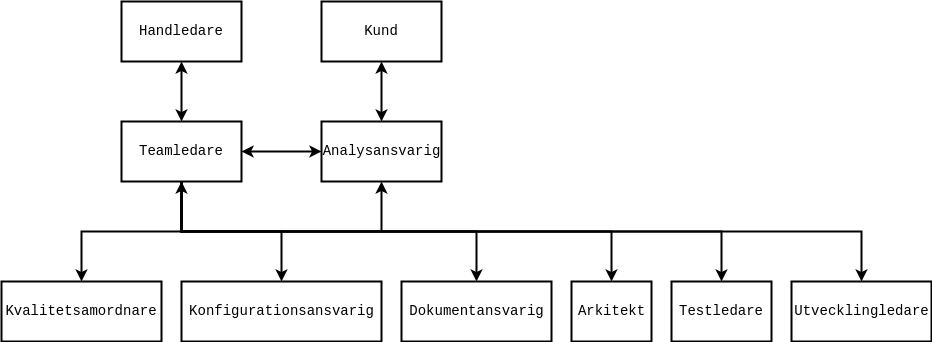
\includegraphics[scale=0.4]{struktur}
    \caption{Projektstruktur}
    \label{fig:struktur}
\end{figure}\\
Gruppen har också skrivit ett gruppkontrakt\cite{bib-gruppkontrakt} som alla gått med på att följa.


\subsection{Roller}
\begin{center}
    \begin{tabular}{| l | l |}
        \hline
        \textbf{Namn} & \textbf{Roll} \\
        \hline
        \centering Alexander Wilkens & Teamledare\\
        \hline
        \centering Joel Almqvist & Kvalitetssamordnare\\
        \hline
        \centering Tim Håkansson & Dokumentansvarig\\
        \hline
        \centering Joel Oskarsson & Arkitekt\\
        \hline
        \centering Lieth Wahid & Utvecklingsledare\\
        \hline
        \centering Axel Löjdquist & Analysansvarig\\
        \hline
        \centering David Kjellström & Testledare\\
        \hline
        \centering Björn Detterfelt & Konfigurationsansvarig\\
        \hline
    \end{tabular}
\end{center}
\subsubsection*{Teamledare}
Teamledaren ska se till att samtliga processer som ska utföras i projektets gång följs. Denna person representerar också gruppen utåt och har kontakt med handledaren. Om det behövs har teamledaren sista ordet.

\subsubsection*{Kvalitetssamordnare}
Ansvarar för arbetsprocesser som ska hålla kvalitén av projektet på en hög nivå. Gör en budget av vad kvalitet får kosta och ansvarar för kvalitetsplanen.

\subsubsection*{Dokumentansvarig}
Ser till att ansvara för samtliga dokument som gruppen ska producera. Även ansvarig för gruppens logotyp och dokumentmallar.

\subsubsection*{Arkitekt}
Ansvarar för att arkitekturen av den tekniska delen av projektet. Gör övergripande teknikval och har det sista ordet på tekniska beslut.

\subsubsection*{Utvecklingsledare}
Ansvarar för den mer detaljerade designen av den tekniska produkten. Leder utvecklingsarbetet och ser till att resten av gruppen har något att arbeta med.

\subsubsection*{Analysansvarig}
Ansvarar för majoriteten av kundkontakt och jobbar ständigt med att ta reda på kundens verkliga behov. Har huvudansvar för kravspecifikationen.

\subsubsection*{Testledare}
Beslutar systemets status genom att arbeta tillsammans med kvalitetssamordnaren för att testa så systemet uppnår kraven. Skriver testplan och testrapport.

\subsubsection*{Konfigurationsansvarig}
Ansvarar för generell versionshantering i projektet. Arbetar mycket med utvecklingledaren och dokumentansvarig för att bestämma vilka arbetsprodukter som ska ingå i en utgåva(release).


\subsection{Kunskap och erfarenheter}
Alla projektmedlemmar har läst flera år på cilivingenjörsprogrammet i datateknik respektive mjukvaruteknik. Gruppen förväntas ha kunskaper och erfarenheter från de tidigare kurser och projekt som utförs i utbildning. Extra fokus ligger på de kurser som studiehandboken listar som förkunskapskrav till TDDD96\cite{bib-tddd96}.


\subsection{Utbildning}
Mycket av den kunskap som gruppen kommer behöva ha för att utföra projektet kommer införskaffas via självstudier. Innan implementationsdelen av projekt drar igång kommer gruppen också få chans att ha en genomgång av Cybercoms API och backend.
\\
Varje projektmedlem är också ansvarig för att sätta sig in i eventuella ramverk och andra tekniker som ska användas i den kommande sprinten.

\subsection{Kommunikation och rapporting}
Gruppen ska under projektets gång producera veckorapporter som ska lämnas in till handledare senast måndag varje vecka. Veckorrapporten beskriver vad gruppen jobbat med under den senaste veckan, vad de ska jobba med i veckan som kommer samt eventuella risker som finns som kan på något sätt hindra projektet. Innan rapporten skickas in ska gruppen ha möte för att bestämma innehållet och diskutera arbete inför veckan. En uppdaterad tidsrapport bifogas också.\\
\\
Kommunikationen i gruppen sker antingen i person eller via Slack. Kommunikation mellan gruppen och handledaren sker via mail genom teamledaren. Kundkommunikation sker antingen i Slack eller via mail genom analysansvarig.

\pagebreak

\section{Risker och riskhantering}
Inom projektet behövs risker frambringas och evalueras för att få så lite motstånd som möjligt. 
Magnituden hos dessa risker beräknas genom produkten utav sannolikheten och inverkan.
Riskerna inför projektet är nedan:

\risk{Cybercoms backend för långsam för våra krav}{1}{4}
{
    För att minimera inverkan på risken så ska backenden användas så lite som möjligt.
    Backended kommer inte att fungera som en fat-server där den utför mycket beräkningar, utan all ''serverkod'' kommer ligga på UI:n. 
    Om det skulle visa sig att backenden fortfarande inte klarar av att skicka information tillräckligt snabbt, 
    så skulle en lösning vara att få spelet att gå långsammare beträffande kontroller.
}

\risk{Sensordata varierar mycket mellan enheter}{2}{2}
{
    Om sensordatan varierar mycket mellan olika enheter, såsom precision eller brus,
    kan det leda till att utvecklingen blir långsammare då det kan ge oönskade problem som måste jobbas runt.
    För att undvika att detta blir ett problem så behövs tydligt efterforskning om hur enheterna fungerar när
    det gäller sensordata. För att fixa problemet om det skulle bli ett behövs koden struktureras upp för att
    hantera problemen tidigt, såsom att motverka brus genom interpolation.
}

\risk{Projektmedlemmar saknar laptops}{1}{3}
{
    Två projektmedlemmar saknar laptops i teamet vilket kan tillföra med att utvecklingen tar längre tid
    då dessa eventuellt får sitta tillsammans med någon annan.
    Cybercom kommer förhoppningsvis att ordna två laptops som kan användas utav medlemmarna, men om det skulle
    visa sig vara ett problem kan medlemmarna utveckla mer i SU-salar med eller utan de andra.
}

\risk{Körtidsfel i JavaScript ger dålig utveckling}{3}{2}
{
    Under projektets gång kommer troligviss JavaScript att ge upphov till oförutsädda körtidsfel då språket inte är typat.
    Detta kan leda till långsammare utveckling då konstiga problem måste letas upp.
    Genom att skapa bra tester kan detta problemet minskas då testerna ska utformas så att oönskade typer hittas snabbt.
    Om problemen kvarstår ska mer resurser läggas på att testerna fungerar.
}

\risk{Arkitekturen lämpar sig inte för realtid}{1}{4}
{
    Då projektets största krav är att spelet ska vara i realtid är det viktigt att arkitekturen fungerar till just
    detta endamålet.
    För att mitigera risken kommer det läggas fokus på arkitekturen i början för att den ska klara av realtid, 
    men även tillsammans hålla koll så att arkitekturen följs.
    Skulle det vissa sig att våran arkitektur ändå inte håller så ska vi så snabbt som möjligt titta över den och bygga om.
}

\risk{Teamledare åker bort en vecka som leder till dålig utveckling}{1}{2}
{
    Då teamledaren lämnar en vecka i slutet utav april kan det leda till att utvecklingen kan
    hindras. För att undvika att detta blir ett problem ska teamledaren hålla alla andra i
    teamet uppdaterade på diverse områden som andra i teamet inte har koll på. I fallet då det skulle bli
    problematiskt finns det inte så mycket att göra, då teamledaren eventuellt inte kan ha någon form utav kontakt,
    teamet får med andra ord jobba på så gott det gå under veckan.
}

\risk{Någon i teamet respekterar inte deadlines}{1}{3}
{
   I alla projekt i team finns det en risk att vissa inte respektera deadlines, både interna och
   externa. För att mitigera detta så kommer teamet se till att alla är uppdaterade på
   diverse deadlines och att på möten hålla koll på vilka som halkar efter. Om det skulle bli
   ett problem ska det tas upp med personen i fråga, om det inte hjälper kontaktar vi handledaren
   eller eventuellt examinatorn för råd.
}

\risk{Oförutsedd dataförlust}{1}{4}
{
    En sak som inte får hända under projektets gång är att all kod eller data försvinner och 
    inte går att få tillbaka. Ett enkelt sätt att undvika att vi förlorar kod är att regelbundet
    versionshantera sin kod med git, även om den inte fungerar så ska den finnas i en personlig
    branch. Detta leder till att kod alltid finns utanför ens personliga dator och därmed mindre
    chans för förlust. Om det skulle vara ett problem med förlust så kan teamet endast gå 
    tillbaka till en tidigare version och fortsätta därifrån.
}

\risk{Saker som inte fungerar blir pushat till master}{1}{3}
{
    Tanken med master-branchen är att allt ska vara körbart och fungera korrekt, så om teamet ska
    demonstrera projektet ska allt köras som tänkt. För att hålla master-branchen fungerande
    kommer tester sättas upp på git som behöver gå igenom för att bli pushat. Dessutom kommer
    konfigurationsansvarig att behöva godkänna pull requests till mastern. Vid problem kan teamet
    gå tillbaka till en tidigare version på mastern vid demonstration och därefter utöka tester
    för att minimera risken att det händer igen.
}

\risk{Brist på kunskap ger dålig kommunikation}{2}{3}
{
   När teamet diskutera saker finns det risk till att vissa i teamet inte har tillräckligt med
   kunskap inom ämnet för att leda en meningsfull diskussion, vilket kan leda till missförstånd
   eller att personen inte medför till diskussionen. Genom att hålla redan i början utav
   projektet ha en uppfattning om vilka erfarenheter teamet har kan teamet bättre förberedda sig
   inför diskussionen. Personen i fråga ska även meddela när det kommer upp ämnen som den inte
   har erfarenheter utav. Vid tillfället då en person har problem och inte meddela detta så
   ska teamet hålla koll så att alla tillför till diskusionen.
}

\pagebreak


\printbibliography
\addcontentsline{toc}{section}{\refname}

\end{document}
